%-----------------------------------------------------------------------------------------------------------------------------------------------%
%	The MIT License (MIT)
%
%	Copyright (c) 2015 Jan Küster
%
%	Permission is hereby granted, free of charge, to any person obtaining a copy
%	of this software and associated documentation files (the "Software"), to deal
%	in the Software without restriction, including without limitation the rights
%	to use, copy, modify, merge, publish, distribute, sublicense, and/or sell
%	copies of the Software, and to permit persons to whom the Software is
%	furnished to do so, subject to the following conditions:
%	
%	THE SOFTWARE IS PROVIDED "AS IS", WITHOUT WARRANTY OF ANY KIND, EXPRESS OR
%	IMPLIED, INCLUDING BUT NOT LIMITED TO THE WARRANTIES OF MERCHANTABILITY,
%	FITNESS FOR A PARTICULAR PURPOSE AND NONINFRINGEMENT. IN NO EVENT SHALL THE
%	AUTHORS OR COPYRIGHT HOLDERS BE LIABLE FOR ANY CLAIM, DAMAGES OR OTHER
%	LIABILITY, WHETHER IN AN ACTION OF CONTRACT, TORT OR OTHERWISE, ARISING FROM,
%	OUT OF OR IN CONNECTION WITH THE SOFTWARE OR THE USE OR OTHER DEALINGS IN
%	THE SOFTWARE.
%	
%
%-----------------------------------------------------------------------------------------------------------------------------------------------%


%============================================================================%
%
%	DOCUMENT DEFINITION
%
%============================================================================%

%we use article class because we want to fully customize the page and dont use a cv template
\documentclass[10pt,A4]{article}	


%----------------------------------------------------------------------------------------
%	ENCODING
%----------------------------------------------------------------------------------------

%we use utf8 since we want to build from any machine
\usepackage[utf8]{inputenc}		

%----------------------------------------------------------------------------------------
%	LOGIC
%----------------------------------------------------------------------------------------

% provides \isempty test
\usepackage{xifthen}

%----------------------------------------------------------------------------------------
%	FONT
%----------------------------------------------------------------------------------------

% some tex-live fonts - choose your own

%\usepackage[defaultsans]{droidsans}
%\usepackage[default]{comfortaa}
%\usepackage{cmbright}
\usepackage[default]{raleway}
%\usepackage{fetamont}
%\usepackage[default]{gillius}
%\usepackage[light,math]{iwona}
%\usepackage[thin]{roboto} 

% set font default
\renewcommand*\familydefault{\sfdefault} 	
\usepackage[T1]{fontenc}

% more font size definitions
\usepackage{moresize}		


%----------------------------------------------------------------------------------------
%	PAGE LAYOUT  DEFINITIONS
%----------------------------------------------------------------------------------------

%debug page outer frames
%\usepackage{showframe}			


%define page styles using geometry
\usepackage[a4paper]{geometry}		

% for example, change the margins to 2 inches all round
\geometry{top=.5cm, bottom=-.6cm, left=-0.1cm, right=0cm} 	

%use customized header
\usepackage{fancyhdr}				
\pagestyle{fancy}

%less space between header and content
\setlength{\headheight}{-5pt}		


%customize entries left, center and right
\lhead{}
\chead{}
\rhead{}

\newcommand{\padding}{1cm}
\newcommand{\innerwidth}{\linewidth-\padding-\padding}

%indentation is zero
\setlength{\parindent}{0mm}

%----------------------------------------------------------------------------------------
%	TABLE /ARRAY DEFINITIONS
%---------------------------------------------------------------------------------------- 

%for layouting tables
\usepackage{multicol}			
\usepackage{multirow}

%extended aligning of tabular cells
\usepackage{array}

\newcolumntype{x}[1]{%
>{\raggedleft\hspace{0pt}}p{#1}}%


%----------------------------------------------------------------------------------------
%	GRAPHICS DEFINITIONS
%---------------------------------------------------------------------------------------- 

%for header image
\usepackage{graphicx}

%for floating figures
\usepackage{wrapfig}
\usepackage{float}
%\floatstyle{boxed} 
%\restylefloat{figure}

%for drawing graphics		
\usepackage{tikz}				
\usetikzlibrary{shapes, backgrounds,mindmap, trees}


%----------------------------------------------------------------------------------------
%	Color DEFINITIONS
%---------------------------------------------------------------------------------------- 
\usepackage{transparent}
\usepackage{color}

%accent color
\definecolor{sectcol}{RGB}{255,150,0}

%dark background color
\definecolor{bgcol}{RGB}{110,110,110}

%light background / accent color
\definecolor{softcol}{RGB}{225,225,225}

% light bg
\definecolor{light}{RGB}{210, 210, 210}

%============================================================================%
%
%
%	DEFINITIONS
%
%
%============================================================================%

%----------------------------------------------------------------------------------------
% 	HEADER
%----------------------------------------------------------------------------------------

% remove top header line
\renewcommand{\headrulewidth}{0pt} 

%remove botttom header line
\renewcommand{\footrulewidth}{0pt}	  	

%remove pagenum
\renewcommand{\thepage}{}	

%remove section num		
\renewcommand{\thesection}{}			

%----------------------------------------------------------------------------------------
% 	ARROW GRAPHICS in Tikz
%----------------------------------------------------------------------------------------

% a six pointed arrow poiting to the left
\newcommand{\tzlarrow}{(0,0) -- (0.2,0) -- (0.3,0.2) -- (0.2,0.4) -- (0,0.4) -- (0.1,0.2) -- cycle;}	

% include the left arrow into a tikz picture
% param1: fill color
%
\newcommand{\larrow}[1]
{\begin{tikzpicture}[scale=0.58]
	 \filldraw[fill=#1!100,draw=#1!100!black]  \tzlarrow
 \end{tikzpicture}
}

% a six pointed arrow poiting to the right
\newcommand{\tzrarrow}{ (0,0.2) -- (0.1,0) -- (0.3,0) -- (0.2,0.2) -- (0.3,0.4) -- (0.1,0.4) -- cycle;}

% include the right arrow into a tikz picture
% param1: fill color
%
\newcommand{\rarrow}[1]
{\begin{tikzpicture}[scale=0.7]
	 \filldraw[fill=#1!100,draw=#1!100!black]  \tzrarrow
 \end{tikzpicture}
}



%----------------------------------------------------------------------------------------
%	custom sections
%----------------------------------------------------------------------------------------

% create a coloured box with arrow and title as cv section headline
% param 1: section title
%
\newcommand{\cvsection}[1]
{
\colorbox{sectcol}{\mystrut \makebox[1\linewidth][l]{
\larrow{bgcol} \hspace{-8pt} \larrow{bgcol} \hspace{-8pt} \larrow{bgcol} \textcolor{white}{\textbf{#1}}\hspace{4pt}
}}\\
}

%create a coloured arrow with title as cv meta section section
% param 1: meta section title
%
\newcommand{\metasection}[2]
{
\begin{tabular*}{1\textwidth}{p{2.5cm} p{11cm}}
\larrow{bgcol}	\normalsize{\textcolor{sectcol}{#1}}&#2\\[8pt]
\end{tabular*}
}

%----------------------------------------------------------------------------------------
%	 CV EVENT
%----------------------------------------------------------------------------------------

% creates a stretched box as cv entry headline followed by two paragraphs about 
% the work you did
% param 1:	event time i.e. 2014 or 2011-2014 etc.
% param 2:	event name (what did you do?)
% param 3:	institution (where did you work / study)
% param 4:	what was your position
% param 5:	some words about your contributions
%
\newcommand{\cvevent}[5]
{
\vspace{8pt}
	\begin{tabular*}{0.8\linewidth}{ p{14cm} x{3cm}}
\textbf{#2} \textcolor{bgcol}{(#3)}&\textcolor{bgcol}{#1}\\[4pt]
	\end{tabular*}
\vspace{-12pt}
\textcolor{softcol}{\hrule}
\vspace{6pt}
	\begin{tabular*}{1\textwidth}{l}
		 \larrow{sectcol}  #4\\[4.5pt]
		 \larrow{sectcol}  #5\\[6pt]
	\end{tabular*}
\vspace{-4pt}
}

\newcommand{\cveventoneline}[5]
{
\vspace{8pt}
	\begin{tabular*}{0.8\linewidth}{ p{14cm} x{3cm}}
\textbf{#2} \textcolor{bgcol}{(#3)}&\textcolor{bgcol}{#1}\\[4pt]
	\end{tabular*}
\vspace{-12pt}
\textcolor{softcol}{\hrule}
\vspace{6pt}
	\begin{tabular*}{1\textwidth}{l}
		 \larrow{sectcol}  #4\\[4.5pt]
	\end{tabular*}
\vspace{-4pt}
}

\newcommand{\cveventthreelines}[6]
{
\vspace{8pt}
	\begin{tabular*}{0.8\linewidth}{ p{14cm} x{3cm}}
\textbf{#2} \textcolor{bgcol}{(#3)}&\textcolor{bgcol}{#1}\\[4pt]
	\end{tabular*}
\vspace{-12pt}
\textcolor{softcol}{\hrule}
\vspace{6pt}
	\begin{tabular*}{1\textwidth}{l}
		 \larrow{sectcol}  #4\\[4.5pt]
		 \larrow{sectcol}  #5\\[4.5pt]
		 \larrow{sectcol}  #6\\[4.5pt]
	\end{tabular*}
\vspace{-4pt}
}

% creates a stretched box as 
\newcommand{\cveventmeta}[2]
{
	\mbox{\mystrut \hspace{87pt}\textit{#1}}\\
	#2
}

%----------------------------------------------------------------------------------------
% CUSTOM STRUT FOR EMPTY BOXES
%----------------------------------------- -----------------------------------------------
\newcommand{\mystrut}{\rule[-.3\baselineskip]{0pt}{\baselineskip}}

%----------------------------------------------------------------------------------------
% CUSTOM LOREM IPSUM
%----------------------------------------------------------------------------------------
\newcommand{\lorem}
{Lorem ipsum dolor sit amet, consectetur adipiscing elit. Donec a diam lectus.}



%============================================================================%
%
%
%
%	DOCUMENT CONTENT
%
%
%
%============================================================================%
\begin{document}

%use our custom fancy header definitions
\pagestyle{fancy}	

%----------------------------------------------------------------------------------------
% HEADLINE / BASIC INFORMATION
%----------------------------------------------------------------------------------------
\fcolorbox{bgcol}{bgcol}{
\begin{minipage}[c][0.085\textheight][t]{\linewidth}
\begin{center}
	\vspace{14pt}
	\textcolor{light}{\small{Devops / Database Engineer $\cdot$  Sydney, Australia  $\cdot$  maiconrocha@gmail.com  $\cdot$ +61 0406 023 410}}\\
	\HUGE{\textcolor{white}{\textsc{Maicon Alegre}} } \textcolor{sectcol}{\rule[-1mm]{1mm}{0.9cm}} \HUGE{\textcolor{white}{\textsc{Resume}} }
\end{center}
\end{minipage}}\\[-4pt]
%----------------------------------------------------------------------------------------
% SUMMARY
%----------------------------------------------------------------------------------------
\fcolorbox{sectcol}{sectcol}{
\begin{minipage}[c][0.03\textheight][t]{\linewidth}
\vspace{-2pt}
\begin{center}
\parbox[b]{0.75\linewidth}{
	\begin{center}
	\large
	\larrow{bgcol}\larrow{bgcol} \textcolor{white}{I'm addicted to learn.} \rarrow{bgcol}\rarrow{bgcol}
	\end{center}
}
\end{center}
\end{minipage}}\\[-4pt]
%----------------------------------------------------------------------------------------
% META
%----------------------------------------------------------------------------------------
\fcolorbox{white}{white}{
\begin{minipage}[c][0.175\textheight][t]{\linewidth}
\vspace{1pt}
\begin{center}
\parbox[c]{\innerwidth}{
	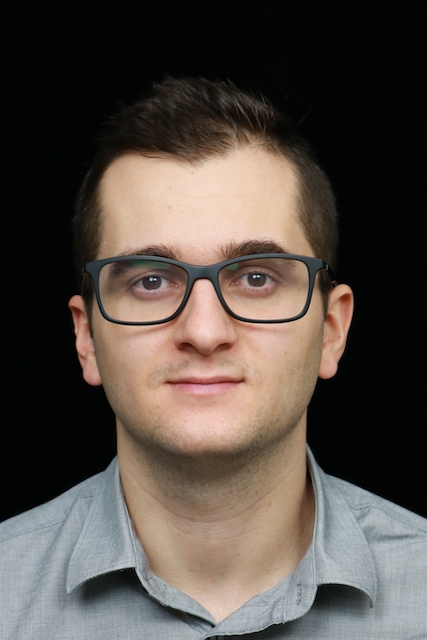
\includegraphics[clip,width=0.16\textwidth]{myfoto.jpg}
	\hspace{10pt}
	\parbox[b]{10cm}{
	\metasection{Summary:}{I am a Cloud Administrator focused on distributed cloud­-based systems, automation and deployment.
Currently, I'm working at AWS as a Cloud Support Engineer, more specifically on Deployment Team.
I have experience in provisioning, operating, maintaining systems running on AWS and also migrating workloads to the cloud. Over 3 years experience as Oracle DBA, and also over 4 years experience as System Analyst and Oracle Developer working on large projects. 

}
	\vspace{-1pt}
	\metasection{Certifications:}{
           
\includegraphics[width=0.06\textwidth]{cka.png}  
\includegraphics[width=0.06\textwidth]{ckad.png} 
\includegraphics[width=0.06\textwidth]{da.png} 
\includegraphics[width=0.06\textwidth]{saa.png} 
\includegraphics[width=0.06\textwidth]{sysop.png} 
\includegraphics[width=0.06\textwidth]{sap.png} 
\includegraphics[width=0.06\textwidth]{devops.png} 
\includegraphics[width=0.06\textwidth]{sec.png}
	}
        }
}
\end{center}
\end{minipage}}\\[-4pt]
%----------------------------------------------------------------------------------------
% EXPERIENCE
%----------------------------------------------------------------------------------------
\fcolorbox{light}{light}{
\begin{minipage}[c][0.55\textheight][t]{\linewidth}
\vspace{4pt}
\hspace{30pt}
\parbox[c]{0.85\linewidth}{
%
\cvevent{2019 - now}{Cloud Support Engineer (Devops)}{AWS - Australia}{Supporting and providing solutions using AWS Deployment Services: ECS/Fargate, EKS, Beanstalk} {CloudFormation, Code(Build, Commit, Deploy, Pipeline), OpsWorks, X-Ray and AppMesh.}

%\textcolor{softcol}{\hrule}

%
\cveventthreelines{2017 - 2018}{Cloud Support Engineer (Databases)}{AWS - Australia}
{AWS DMS(Database Migration Service) SME}
{Supporting and providing solutions using RDS MySQL/MariaDB, Oracle} {Aurora(MySQL/PostgreSQL), PostgreSQL and SQL Server}


%\textcolor{softcol}{\hrule}

%
\cvevent{2015 - 2016}{Cloud SysOp Administrator}{ilegra(https://ilegra.com/en/) - Brazil}{Deploy, manage, and operate scalable, highly available, and fault tolerant systems on AWS Cloud}{Migrate an existing on-premises application to AWS Cloud/Automation and development using Python}

%\textcolor{softcol}{\hrule}

%
\cveventthreelines{2014 - 2015}{DBA/Middleware Analyst}{ilegra(https://ilegra.com/en/) - Brazil}{Oracle Database Administration (10g, 11g, 12c), MySQL, MongoDB, SQLServer}{Topics included installation, automation, administration, migration, tuning}{Deployment of applications, diagnosis and troubleshooting, provide support for development team}

%\textcolor{softcol}{\hrule}

%
\cvevent{2012 - 2014}{Oracle DBA/Developer}{ilegra(https://ilegra.com/en/) - Brazil}{Oracle Database Administration (10g, 11g)}{Topics included installation, automation, administration, migration, tuning, development(PL/SQL, Bash script)}

%\textcolor{softcol}{\hrule}


%
\cveventoneline{2011 - 2012}{Oracle Analyst/Developer}{Sonda(https://www.sonda.com/en/) - Brazil)}{Working as a consultant Oracle Analyst / Developer}

%\textcolor{softcol}{\hrule}


%
\cveventoneline{2010 - 2011}{Oracle Developer}{ilegra(https://ilegra.com/en/) - Brazil}{Development and automation using PL/SQL}

%\textcolor{softcol}{\hrule}


%
\cveventoneline{2008 - 2010}{Oracle Developer}{CWI Software(https://cwi.com.br/) - Brazil}{Working exclusively for Walmart - Development and automation using PL/SQL}

}
\hspace{2pt}
\textcolor{sectcol}{\rule[-3.2cm]{1pt}{7cm}}
\hspace{2pt}
\rotatebox[origin=c]{270}{\large \textsc{Experience}}
\end{minipage}}\\[-1pt]
%----------------------------------------------------------------------------------------
% SUMMARY
%----------------------------------------------------------------------------------------
\fcolorbox{bgcol}{bgcol}{
\begin{minipage}[c][0.01\textheight][t]{\linewidth}
\vspace{-1pt}
\begin{center}
\parbox[b]{0.75\linewidth}{
%	\begin{center}
%	 	\textcolor{white}{https://www.linkedin.com/in/maicon-alegre-010bb116/ - } \textcolor{white}{https://github.com/maiconrocha}
%	\end{center}
}
\end{center}
\end{minipage}}
%----------------------------------------------------------------------------------------
% EDUCATION
%----------------------------------------------------------------------------------------
\fcolorbox{white}{white}{
\begin{minipage}[c][0.09\textheight][t]{\linewidth}
\vspace{1pt}
\hspace{26pt}
\parbox[c]{0.85\linewidth}{
\cvevent{2006 - 2012}{Bachelor of Computer Information Systems}{Unisinos - Brazil}{Master Thesis: Case Study: Lean and Agile Methodologies during} {stabilization phase of a software system}
}
\hspace{2pt}
\textcolor{sectcol}{\rule[-1.5cm]{1pt}{3cm}}
\hspace{2pt}
\rotatebox[origin=c]{270}{\large \textsc{Education}}
\end{minipage}}\\[-0pt]
%---------------------------------------------------------------------------------------
%	QR CODE (optional)
%----------------------------------------------------------------------------------------
%\vspace{-136pt}
%\hspace{0.75\linewidth}
%\includegraphics[width=103pt]{qrcode}
%\normalsize
%\vspace{88pt}



%-------------------------------------------------------------------------------------------------
% FOOTER
%--------------------------------------------------------------------------------------------------
\fcolorbox{bgcol}{bgcol}{
\begin{minipage}[c][0.01\textheight][t]{\linewidth}
\vspace{-8pt}
\begin{center}
\parbox[b]{0.75\linewidth}{
	\begin{center}
	 	\textcolor{white}{https://www.linkedin.com/in/maicon-alegre-010bb116/ - } \textcolor{white}{https://github.com/maiconrocha}
	\end{center}
}
\end{center}
\end{minipage}}
%============================================================================%
%
%
%
%	DOCUMENT END
%
%
%
%============================================================================%
\end{document}
